\documentclass[doc,natbib,floatsintext]{apa7}

\usepackage{lipsum}
\usepackage{graphics}
\graphicspath{
{figures/}
}

\title{Title}
\shorttitle{Short title}

\author{Authorname}
\affiliation{Affiliation}

\leftheader{Lastname}

\abstract{\lipsum[1]}

\keywords{some keywords}

\authornote{Some info about the author}

% DOCUMENT BEGINS 
\begin{document}

\maketitle

\section{Introduction} 

Here is where the introduction would go. 

% I can add some thoughts here as comments and they won't show up in the pdf. 

\subsection{Citations}

Some authors said something interesting \citep{gerstenberg2021csm}. \cite{gelman1986categories} said something even more interesting.

\subsubsection{Another section}

\lipsum[1]

\paragraph{And another section}

\lipsum[1]

\section{Methods}

\subsection{Figures}

This is how you add figures to your document. You can then refer to the figure in text like so (see Figure~\ref{fig:example_figure}). 

\begin{figure}[t]
    \centering
    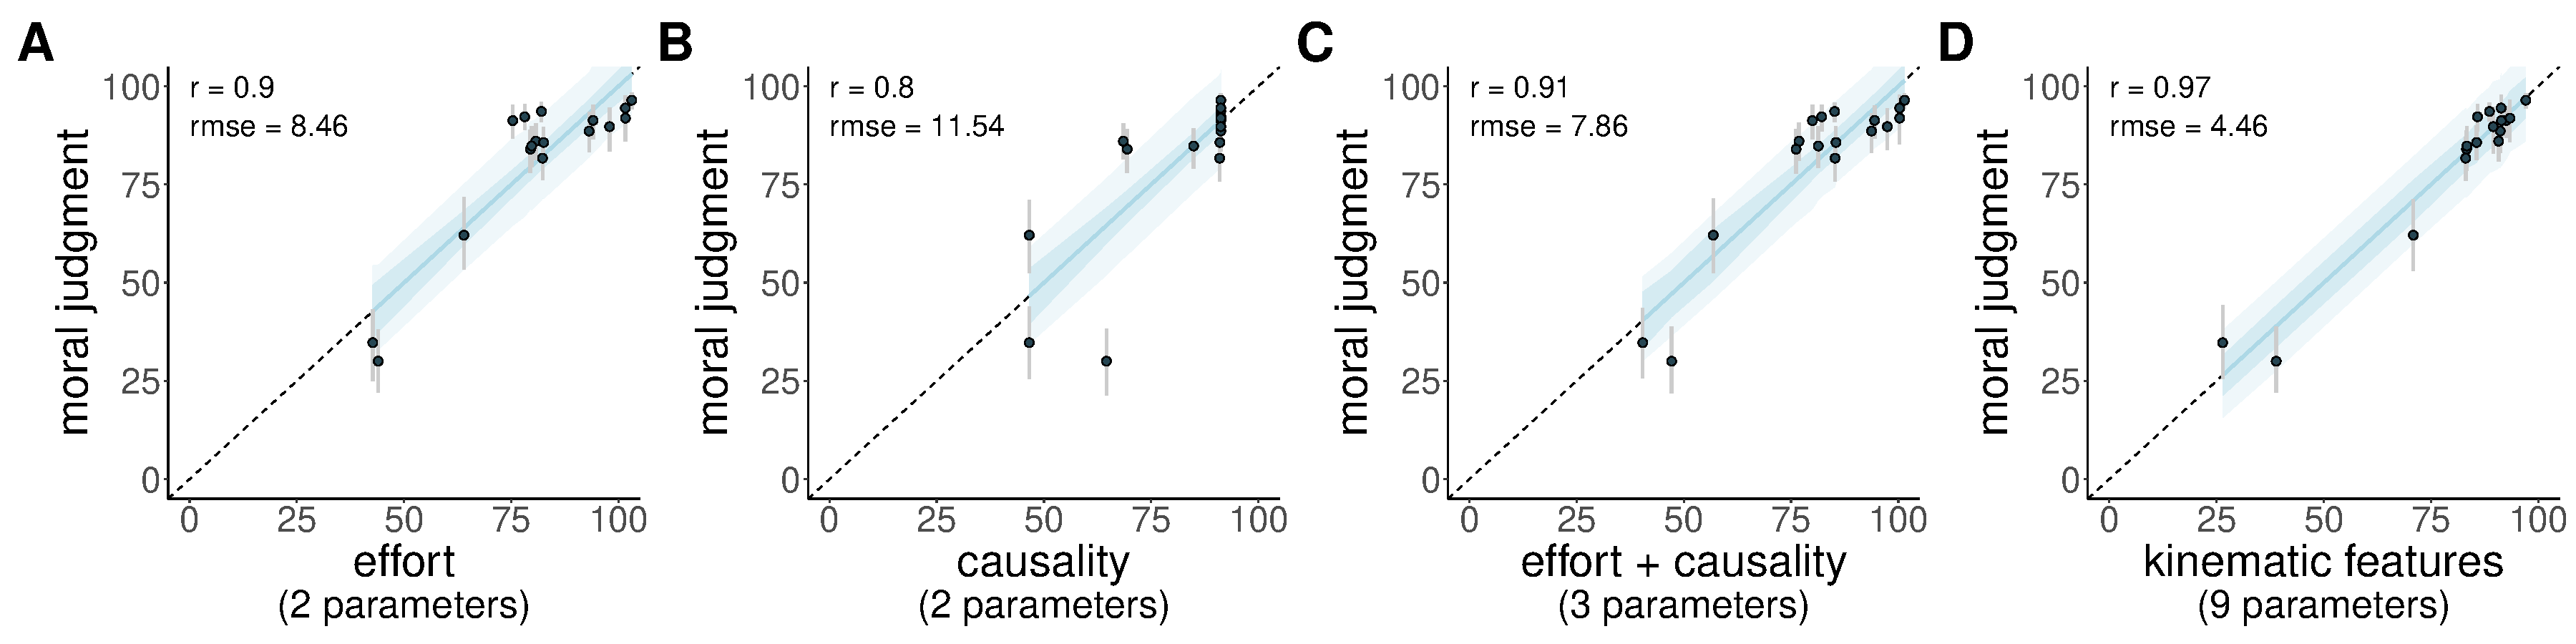
\includegraphics[width=0.99\columnwidth]{example_figure}
    \caption{An example figure.}
    \label{fig:example_figure}
\end{figure}


\subsection{Tables} 

\url{https://www.tablesgenerator.com/} is helpful for making tables. Table~\ref{tab:simple_table} shows an example table. 

\begin{table}[b]
\caption{A simple table.}
\label{tab:simple_table}
\begin{tabular}{lll}
\toprule
name  & index & value \\
\midrule
steve & 1     & 31    \\
mary  & 2     & 23   \\
\bottomrule
\end{tabular}
\end{table}

% REFERENCES
\clearpage 
\bibliographystyle{apacite}
\bibliography{references}

\end{document}

